\documentclass[a4paper]{article}
%% Jose Javier Gonzalez Ortiz %%
%% Plantilla Latex generica   %%
%% 2014-11-08                 %%


% Generic Pakages
    \usepackage[utf8]{inputenc}                         % For Spanish characters
    \usepackage[english]{babel}               % Spanish hyphenation and document rules
    \usepackage{amsmath}                                % Standard math packages
    \usepackage{graphicx}                               % Image insertion.
    \usepackage{tikz}
    \usepackage{caption,subcaption}                     % For custom caption environments

    \usepackage{booktabs}                               % Beautiful Tables
    \usepackage{hyperref}                               % For linked references and URLinks
    \usepackage{fancyhdr}                               % Custom headers and footers
    \usepackage{appendix}                               % Enables appendices
    \usepackage{pdfpages}                               % Insert pdfs
    \usepackage{array}                                  % Enables array features
    \usepackage{algorithm}
    \usepackage[noend]{algpseudocode}
    \usepackage{eqparbox}
    \makeatletter
    \def\BState{\State\hskip-\ALG@thistlm}
    \makeatother
    %\usepackage[americanvoltages, europeancurrents, americanresistors, cuteinductors]{circuitikz}                          % Circuit Graphics
    \usepackage{mathtools}
    \usepackage{amsthm}
    
%Additional Features
    \usepackage{lipsum}                                 % Used for inserting dummy 'Lorem ipsum' text into the template
    \usepackage{enumerate}                              % Custom numerate, useful for i,ii,iii... I,II,III...
    \usepackage{sectsty}                                % Allows customizing section commands
    \usepackage{todonotes}                              % useful for leaving todonotes
    \usepackage[space]{grffile}                         % insert files with spaces
     %\usepackage{microtype}                             % Beatify engine
    %\usepackage[superscript]{cite}                     % CIting with superscript numerals
    %\usepackage{xcolor}                                    % Required for inserting color
    %\usepackage[usenames,dvipsnames]{color}                % Required for custom colors
    %\usepackage{xargs}                                 % Expanded arguments features
    %\usepackage{fix-cm}                                 % Computer-Modern at arbitrarysizes
    \usepackage{siunitx}                               % For SI Units
    %\usepackage{eurosym}                                % Eurosymbol
    %\usepackage{pdflscape}                              % enables landscape for pdfs
    %\usepackage{longtable}                              % Tables than span multipages

% Custom Settings
    % \decimalpoint                                       % American Decimal Point instead of Spanish comma

    % Margins
        \topmargin      = -0.45in
        \evensidemargin = 0in
        \oddsidemargin  = 0in
        \textwidth      = 6.5in
        \textheight     = 9.0in
        \headsep        = 0.25in

    \pagestyle{fancy}
    \lhead{\HWAuthorName}
    \chead{}
    \rhead{\HWClass : \HWTitle}
    \lfoot{}
    \cfoot{\thepage}
    \rfoot{}
    
    \renewcommand\headrulewidth{0.4pt} % Size of the header rule
    \renewcommand\footrulewidth{0.4pt} % Size of the footer rule

    \numberwithin{equation}{section} % Number equations within sections (i.e. 1.1, 1.2, 2.1, 2.2 instead of 1, 2, 3, 4)
    \numberwithin{figure}{section} % Number figures within sections (i.e. 1.1, 1.2, 2.1, 2.2 instead of 1, 2, 3, 4)
    \numberwithin{table}{section} % Number tables within sections (i.e. 1.1, 1.2, 2.1, 2.2 instead of 1, 2, 3, 4)

    \renewcommand{\labelitemi}{$\bullet$}                       %%bullet1 circle
    \renewcommand{\labelitemii}{\leavevmode \hbox to
    1.2ex {\hss \vrule height .9ex width .7ex depth -.2ex\hss }} %%bullet2 box

    \newcommand{\ul}[1]        {\underline{\smash{#1}}}         %%closer underline
    \newcommand{\gm}[1]         {\guillemotleft #1\guillemotright}  %$ pretty <<sth>>$

    \DeclarePairedDelimiter\floor{\lfloor}{\rfloor}
    \DeclarePairedDelimiter\ceil{\lceil}{\rceil}

%%%%%%%%%%%%%%%%%%%%%%%%%%%%%%%%%%%%%%%%%%%%%%%%%%%%%%%%%%%%%%%%%%%%%%%%%%%%%%%%%%
%%%                             CODIGO                                         %%%
%%%%%%%%%%%%%%%%%%%%%%%%%%%%%%%%%%%%%%%%%%%%%%%%%%%%%%%%%%%%%%%%%%%%%%%%%%%%%%%%%%

% Code insertion
    \usepackage{listings}                               % Main package for inserting code
    \usepackage{courier}                                % For using the courier font

    \AtBeginDocument{\numberwithin{lstlisting}{section}}  % Number listings within sections (i.e. 1.1, 1.2, 2.1, 2.2 instead of 1, 2, 3, 4)
    
    %%\captionsetup[lstlisting]{font={small,tt}}            %  Listings Font Size
    
    \renewcommand{\lstlistingname}{Código}              % For Codigo caption (requires caption package)

    \definecolor{background}{gray}{.98}                 % Background color definition
    \definecolor{comments}{RGB}{51,102,0}               % Comments   color definition
    \definecolor{keywords}{RGB}{0,0,120}                % Keywords   color definition
    \definecolor{keywords2}{RGB}{204,0,102}             % Keywords2  color definition
    \definecolor{numbers}{RGB}{127, 0, 127}             % Keywords2  color definition

    \definecolor{Maroon}{RGB}{128, 0, 0}

       % morekeywords={add,sub,mul,mulu,nand,sll,sra,srl,sltu,addi,sw,lw,beq,jarl,lui},
    \lstdefinelanguage{ICAI-RiSC-16}
   {morekeywords={add,sub,mul,mulu,nand,sll,sra,srl,sltu,addi,sw,lw,beq,jalr,lui,la,med},
        sensitive=false,
        morecomment=[l]{\#},
        morecomment=[l][\color{Maroon}]{.},
        morekeywords=[2]{r0, r1, r2, r3, r4, r5, r6, r7},
        keywordstyle=[2]{\color{violet}},
        % literate=%
        %    *{0}{{{\color{red!20!violet}0}}}1
        %     {1}{{{\color{red!20!violet}1}}}1
        %     {2}{{{\color{red!20!violet}2}}}1
        %     {3}{{{\color{red!20!violet}3}}}1
        %     {4}{{{\color{red!20!violet}4}}}1
        %     {5}{{{\color{red!20!violet}5}}}1
        %     {6}{{{\color{red!20!violet}6}}}1
        %     {7}{{{\color{red!20!violet}7}}}1
        %     {8}{{{\color{red!20!violet}8}}}1
        %     {9}{{{\color{red!20!violet}9}}}1
        %morecomment=[s]{/*}{*/},
        %morestring=[b]"
    }


    \lstset{
        frame=Ltb,
        framerule=0pt,
        aboveskip=0.5cm,
        framextopmargin=3pt,
        framexbottommargin=3pt,
        framexleftmargin=0.4cm,
        framesep=0pt,
        rulesep=.4pt,
        backgroundcolor=\color{background},
        rulesepcolor=\color{black},
        rulecolor=\color{black},
        %
        stringstyle=\ttfamily,
        basicstyle=\small\ttfamily,
        commentstyle=\itshape\color{comments},
        keywordstyle=\bfseries\color{keywords},
        %
        numberstyle=\tiny,
        numbers=left,
        numbersep=15pt,
        numberfirstline = false,
        %
        breakatwhitespace=false,         % sets if automatic breaks should only happenat whitespace
        breaklines=true,                 % sets automatic line breaking
        captionpos=b,                    % sets the caption-position to bottom
        escapeinside={<@}{@>},            % if you want to add LaTeX within your code
        keepspaces=true,                 % keeps spaces in text, useful for keepingindentation of code (possibly needs columns=flexible)
        showspaces=false,                % show spaces everywhere adding particularunderscores; it overrides 'showstringspaces'
        showstringspaces=false,          % underline spaces within strings only
        showtabs=false,                  % show tabs within strings adding particularunderscores
        stepnumber=1,                    % the step between two line-numbers. If it's1, each line will be numbered
        tabsize=2,                       % sets default tabsize to 2 spaces
    }
    

    \lstdefinestyle{customvhdl}{
        language=vhdl,                              % Language
        morekeywords = {},
        morestring=[b][\color{numbers}]',
        morestring=[b][\color{numbers}]",
        emph={std_logic,std_logic_vector,integer,unsigned,to_unsigned},
        emphstyle={\color{keywords2}\bfseries},%
        %deletekeywords={...},            % if you want to delete keywords from the given language
    }

    \lstdefinestyle{customc}{
        language = C
    }

    \lstset{language = ICAI-RiSC-16}



    % Grey scale definitions - Printing
    %\definecolor{background}{gray}{.98}
    %\definecolor{comments}{gray}{.45}
    %\definecolor{keywords}{gray}{.25}


%%%%%%%%%%%%%%%%%%%%%%%%%%%%%%%%%%%%%%%%%%%%%%%%%%%%%%%%%%%%%%%%%%%%%%%%
%%%%%%%%%%%%%%%%%%%%%%       HERE BE DRAGONS        %%%%%%%%%%%%%%%%%%%%
%%%%%%%%%%%%%%%%%%%%%%%%%%%%%%%%%%%%%%%%%%%%%%%%%%%%%%%%%%%%%%%%%%%%%%%%
%
%%%%%%%%%%%%%%%%%%%%%%%%%%%%%%%%%%%%%%%%%%%%%%%%%%%%%%%%%%%%%%%%%%%%%%%%
%%%% Paragraph separation
%\setlength{\parskip}{.5em}
%%%%%%%%%%%%%%%%%%%%%%%%%%%%%%%%%%%%%%%%%%%%%%%%%%%%%%%%%%%%%%%%%%%%%%%%
%%%% Table separation
%\renewcommand{\arraystretch}{1.3}
%%%%%%%%%%%%%%%%%%%%%%%%%%%%%%%%%%%%%%%%%%%%%%%%%%%%%%%%%%%%%%%%%%%%%%%%
%%%% 9+ Arguments functions
%\newcommand{\function}[9]{%
%        \def\tempa{#1}%
%        \def\tempb{#2}%
%        \def\tempc{#3}%
%        \def\tempd{#4}%
%        \def\tempe{#5}%
%        \def\tempf{#6}%
%        \def\tempg{#7}%
%        \def\temph{#8}%
%        \def\tempi{#9}%
%        \functioncont
%    }
%%%%%%%%%%%%%%%%%%%%%%%%%%%%%%%%%%%%%%%%%%%%%%%%%%%%%%%%%%%%%%%%%%%%%%%%
%%%% Rules for longtable
%\newcommand{\mytoprule}{\specialrule{1.5pt}{0em}{0em}}
%\newcommand{\mymidrule}{\specialrule{.75pt}{0em}{0em}}
%\newcommand{\mybottomrule}{\specialrule{1.5pt}{0em}{0em}}
%
%%%%%%%%%%%%%%%%%%%%%%%%%%%%%%%%%%%%%%%%%%%%%%%%%%%%%%%%%%%%%%%%%%%%%%%%
%%%% Roman numerals at the start
%
%\pagenumbering{roman}
%\tableofcontents
%\newpage
%\listoftables
%\newpage
%\pagenumbering{arabic}
%%%%%%%%%%%%%%%%%%%%%%%%%%%%%%%%%%%%%%%%%%%%%%%%%%%%%%%%%%%%%%%%%%%%%%%%
%%%% More than 18 floating figures/tables - force to put
%\clearpage
%%%%%%%%%%%%%%%%%%%%%%%%%%%%%%%%%%%%%%%%%%%%%%%%%%%%%%%%%%%%%%%%%%%%%%%%
%%%% Landscape tables recommendations
%\topmargin      = -0.95in
%\evensidemargin = 0in
%\oddsidemargin  = 0in
%\textwidth      = 6.5in %6.5in
%\textheight     = 9.75in
%\headsep        = 0.25in
%\small  % Switch from 12pt to 11pt
%\setlength\LTleft{0pt}            % default: \parindent
%\setlength\LTright{0pt}           % default: \fill
%%%%%%%%%%%%%%%%%%%%%%%%%%%%%%%%%%%%%%%%%%%%%%%%%%%%%%%%%%%%%%%%%%%%%%%%
%%%% Bold columns table
%>{\bfseries\arraybackslash}m{1.1in}
%
%%%%%%%%%%%%%%%%%%%%%%%%%%%%%%%%%%%%%%%%%%%%%%%%%%%%%%%%%%%%%%%%%%%%%%%%
%%%% \epigraph{}
%
%\makeatletter
%\patchcmd{\epigraph}{\@epitext{#1}}{\itshape\@epitext{#1}}{}{}
%\makeatother
%%%%%%%%%%%%%%%%%%%%%%%%%%%%%%%%%%%%%%%%%%%%%%%%%%%%%%%%%%%%%%%%%%%%%%%%
%%%% Quotes -> chapquote enviroment
%\makeatletter
%\newenvironment{chapquote}[2][2em]
%  {\setlength{\@tempdima}{#1}%
%   \def\chapquote@author{#2}%
%   \parshape 1 \@tempdima \dimexpr\textwidth-2\@tempdima\relax%
%   \itshape}
%  {\par\normalfont\hfill--\ \chapquote@author\hspace*{\@tempdima}\par\bigskip}
%\makeatother
%%%%%%%%%%%%%%%%%%%%%%%%%%%%%%%%%%%%%%%%%%%%%%%%%%%%%%%%%%%%%%%%%%%%%%%%

% Global variables
\newcommand{\tu}           {\underline}
\newcommand{\HWTitle}           {Homework 3}
\newcommand{\HWSubtitle}        {}
\newcommand{\HWDueDate}         {\today}
\newcommand{\HWClass}           {EECS 587 Parallel Computing}
\newcommand{\HWAuthorName}     {José Javier González Ortiz}

\title{\HWTitle \\ \vspace{.25cm} \large\HWSubtitle}
\author{\HWAuthorName}
\date{\HWDueDate}

\setlength{\parskip}{.5em}

\renewcommand\algorithmiccomment[1]{%
  \hfill\ \eqparbox{COMMENT}{#1}%
}

% \DeclarePairedDelimiter\par{\left(}{\right)}

\newcommand\LONGCOMMENT[1]{%
  \hfill\ \begin{minipage}[t]{\eqboxwidth{COMMENT}}#1\strut\end{minipage}%
}

\begin{document}
\maketitle
\thispagestyle{fancy}

\section{Algorithm}
    Given the problem in the assignment we can show that although the initial matrix is symmetrical, after the first iteration we will lose the symmetry so we have to calculate all the values in the matrix.

    Given more processors we can split the work to be done. Since we want the divisions to be as cohesive as possible to minimize the communication, we can opt for two ways to do the domain decomposition. Both involve \emph{Halo Swapping} as it renders the most effective strategy in this case since every element depends on the ones above, below and to the right.

    First the serial time for this algorithm will be SerTime $ = \Theta(n^2)$ since we will do a constant amount of iterations during which it will update the $n^2$ elements of the matrix. Now, an ideal parallel algorithm without communication we would get ParTime $ = \Theta(n^2 / p)$, however any real algorithm will have to communicate so the SpeedUp won't be $p$.

    If we do the division per processors in one dimension, the Parallel time will be as follows: ParTime $= \Theta(n^2/p) + \Theta(n/p) + \Theta(n) = \Theta(n^2/p) + \Theta(n) $. However, if we do the partition in both dimensions (we are allowed to do it since $p$ is given to be a perfect square) the parallel time will be ParTime $= \Theta(n^2/p) + \Theta(n/\sqrt{p})$ which is clearly better than the naive approach shown before.

    % It can be shown that given an fixed rectangular area $S$ of sides $l$ and $S/l$ the minimum perimeter happens when $l = S/l = \sqrt{S}$. In this problem the

\section{Analysis}
    The chosen domain decomposition renders the processor communication in a 2D grid. To better the communication involved there should be communication between the first row of processors and the last row, to make use of the modular properties of the algorithm. Therefore, the sought topology is cylindrical.

    Given the partition shown we will have for each processor $p$ with coordinates in the processor grid $(x,y)$. The size of the matrix will be $h \times w$ where $h$ and $w$ are:
    \begin{align}
    h = \begin{cases}
    \ceil{\frac{n}{\sqrt{p}}} \quad & \text{if  } x < \sqrt{p}-1\\
    n \mod \ceil{\frac{n}{\sqrt{p}}} \quad & \text{if  } x = \sqrt{p}-1\\
    \end{cases}\\
    w = \begin{cases}
    \ceil{\frac{n}{\sqrt{p}}} \quad & \text{if  } y < \sqrt{p}-1\\
    n \mod \ceil{\frac{n}{\sqrt{p}}} \quad & \text{if  } y = \sqrt{p}-1\\
    \end{cases}
    \end{align}

    Apart from this $h \times w$ matrix, each processor will have to store three halos corresponding to the following values
    \begin{itemize}
        \item \textbf{Upper Halo} of size $1 \times w$, corresponding to the lower row of the processor above (note that $(\sqrt{p}-1,y)$) is above $(0,y)$ in a cylindrical topology). This values are needed when $i_{\text{local}} = 0$ and $i''$ looks for the value above.
        \item \textbf{Lower Halo} of size $1 \times w$, corresponding to the upper row of the processor below. This values will be needed hen $i_{\text{local}} = \ceil{\frac{n}{\sqrt{p}}} -1$ and $i'$ looks for the value below.
        \item \textbf{Right Halo} of size $h \times 1$, corresponding to the leftmost column of the processor to the right. This values will be needed when $j_{\text{local}} = \ceil{\frac{n}{\sqrt{p}}} -1$ and $j'$ will ask for the value to the right. The processors with coordinates $(x, \sqrt{p}-1)$ will not use this halos since the values of the matrix with coordinates $(i,n-1)$ do not update.
    \end{itemize}
    The communication will be composed in three shifts.
    \begin{enumerate}
        \item \textbf{Upward Modular Shift} Each processor $(x,y)$ sends its upper row to the processor above $(x -1 \mod \sqrt{p},y)$ and receives from the one below $(x +1 \mod \sqrt{p},y)$ storing the values in the Lower Halo. Since this is a cylindrical topology this operation involves all the processors sending and receiving at the same time.
        \item \textbf{Downward Modular Shift} Similarly, this is the reverse operation. Each processor $(x,y)$ sends its lower row to the processor below $(x +1 \mod \sqrt{p},y)$ and receives from the one above $(x -1 \mod \sqrt{p},y)$ storing the values in the Upper Halo.
        \item \textbf{Leftward Shift} This involves every processor $(x,y)$ sending its leftmost column to the one on their left $(x,y-1)$ side and receiving from the one on their right $(x,y+1)$ and storing th values in their Right Halo. Note than this an open loop and the processors $(x,0)$ won't send any information and the processors $(x,\sqrt{p}-1)$ won't receive any information either.
    \end{enumerate}

    From this we can gather that the communication time is $O(\max(h,w))$ since we are swapping three halos per processor every time the processors communicate. Since $\max(h,w) = \ceil{\frac{n}{\sqrt{p}}}$ the time involved in the communication will be $O(\frac{n}{\sqrt{p}})$.

    Since the update involved modifying the whole matrix it will take time $O(h\times w)$ per processor. Since $h,w \leq \ceil{\frac{n}{\sqrt{p}}}$ we can express it as $O(h\times w) = O(n^2/p)$.

    Finally the whole parallel time will be
    \begin{equation}
        \text{ParTime} = \Theta(n^2/p) + \Theta(n/\sqrt{p})\\
    \end{equation}

    The SpeedUp will be
    \begin{equation}
        \text{SpeedUp} = \frac{\text{SerTime}}{\text{ParTime}} = \frac{\Theta(n^2)}{\Theta(n^2/p) + \Theta(n/\sqrt{p})}
    \end{equation}
    \begin{equation}
        \text{SpeedUp} \rightarrow p \qquad\text{as}\qquad n \rightarrow \infty
        \label{eq:SpeedUp}
    \end{equation}

    And the efficiency:
    \begin{equation}
        \text{Efficiency}  = \frac{\text{SerTime}}{p \cdot \text{ParTime}} = \frac{\Theta(n^2)}{\Theta(n^2) + \Theta(n\sqrt{p})}
    \end{equation}
    \begin{equation}
        \text{Efficiency} \rightarrow 1 \qquad\text{for}\qquad p = O(n^2)
        \label{eq:Efficiency}
    \end{equation}
\newpage
\section{Implementation}
    To implement the algorithm we have used the partition described above and used a cylindrical virtual topology where the row processors are wrapped around but the column processors are not. Furthermore it has been used \texttt{MPI\_SENDRECV} for the communication, using a derived datatype for the column communication.

    The particular aspects of the whole implementation can be seen in Code \ref{cod:matrix}

\section{Results}
    The results from the timings are shown in the Table \ref{tab:Results}. The Verification values for the different matrix sizes are shown in the Table \ref{tab:Verification}.

    \begin{table}[!htp]
      \center
      \begin{tabular}{*{5}{r}}
        \textbf{n} &  \textbf{p} &   \textbf{average} &       \textbf{min} &       \textbf{max} \\
    \midrule
     1000 & 1 & 5.71552 & 5.34630 & 5.83059\\
     2000 & 1 & 22.82041 & 21.18143 & 23.31813\\
     1000 & 4 & 1.46049 & 1.41766 & 1.49389\\
     2000 & 4 & 6.04183 & 5.67908 & 7.35377\\
     1000 & 16 & 0.46770 & 0.38920 & 0.54539\\
     2000 & 16 & 1.77513 & 1.50135 & 2.04136\\
     1000 & 36 & 0.30457 & 0.22946 & 0.37673\\
     2000 & 36 & 1.01406 & 0.68300 & 1.30123\\
      \end{tabular}
      \caption{Results in seconds}
      \label{tab:Results}
    \end{table}
        
    \begin{table}[!htp]
      \center
      \begin{tabular}{*{3}{r}}
        \textbf{n} &   \textbf{sum} &       \textbf{min}\\
    \midrule
     1000 &  4283810.871966  & -892.718330   \\
     2000 & 17631642.148465  & -1800.724437  \\
      \end{tabular}
      \caption{Verification Values}
      \label{tab:Verification}
    \end{table}

    To ease the understanding of the data we can plot different relations between the data. In figures \ref{fig:1000} and \ref{fig:2000} we can see the timing results in a log scale for $n = 1000$ and $n = 2000$. Defining $\text{SerTime}(n) = \text{ParTime}(n,1)$ and calculating the ideal parallel time as $\text{SerTime}/p$ we get some interesting results. As we can see the curves match up quite nicely, being the minimum time better than the average one, which seems logical. The deviation for greater $p$ seems larger, however we are using a log scale so in fact it is not as big of a difference. Finally, we can see that for $n = 2000$ the minimum case does better $n = 1000$.

    \begin{figure}[htp!]
      \centering
      \begin{subfigure}{.5\textwidth}
        \centering
        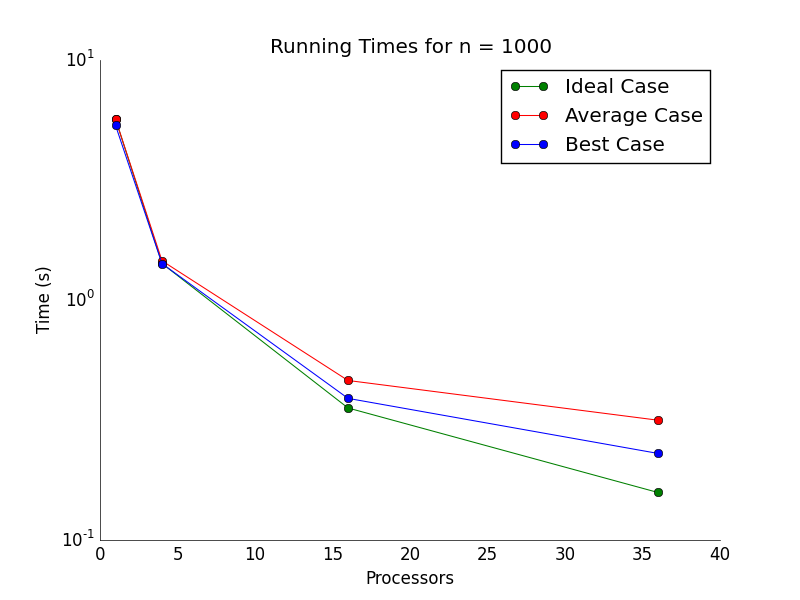
\includegraphics[width=.99\textwidth]{../2 Analysis/1000.png}
        \caption{$n = 1000$}
        \label{fig:1000}
      \end{subfigure}%
      \begin{subfigure}{.5\textwidth}
        \centering
        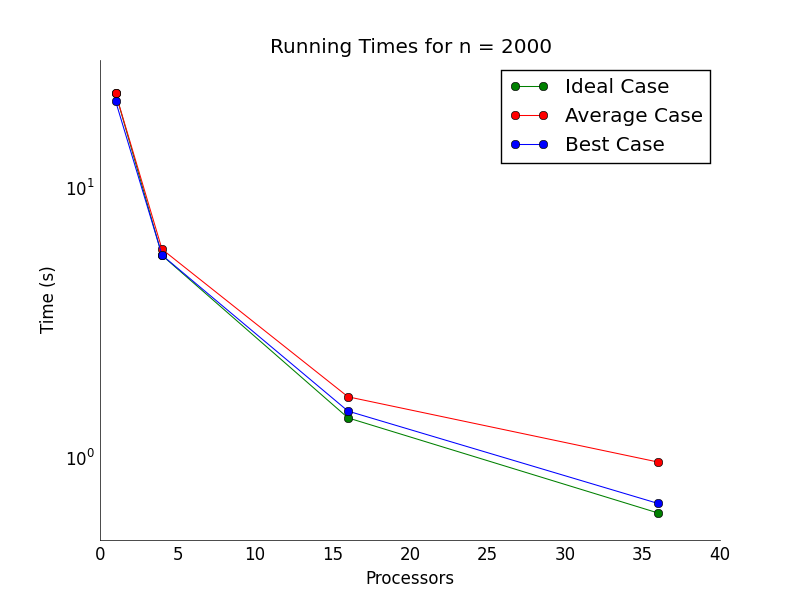
\includegraphics[width=.99\textwidth]{../2 Analysis/2000.png}
        \caption{$n = 2000$}
        \label{fig:2000}
      \end{subfigure}
      \caption{Logarithmic plot of times for different number of processors}
    \end{figure}

    Now, to analyze both SpeedUp and Efficiency, we can see the plots shown in Figures \ref{fig:SpeedUp} and \ref{fig:Efficiency}, in which we can find the ideal case, for $n = 1000$ and for $n = 2000$. In this plots an average of the minimum cases has been used to avoid deviating the data with longer timings.

    Analyzing the Figures we can see that we have achieved almost linear SpeedUp as the Equation \eqref{eq:SpeedUp} predicted. As $n$ goes from $1000$ to $2000$ the SpeedUp improves verifying our predictions. For the Efficiency, Equation \eqref{eq:Efficiency} predicted constant efficiency as $n$ grew larger. Figure \ref{fig:Efficiency} confirms this, with $n = 2000$ having a behavior much closer to ideal efficiency than $n = 1000$.

    Finally, it is important to notice that MPI communication does not behave as the theoretical models and therefore the results will not match perfectly to the model. Nevertheless, we have achieved successful results in the time needed to solve the problem.


    \begin{figure}[htp!]
      \centering
      \begin{subfigure}{.5\textwidth}
        \centering
        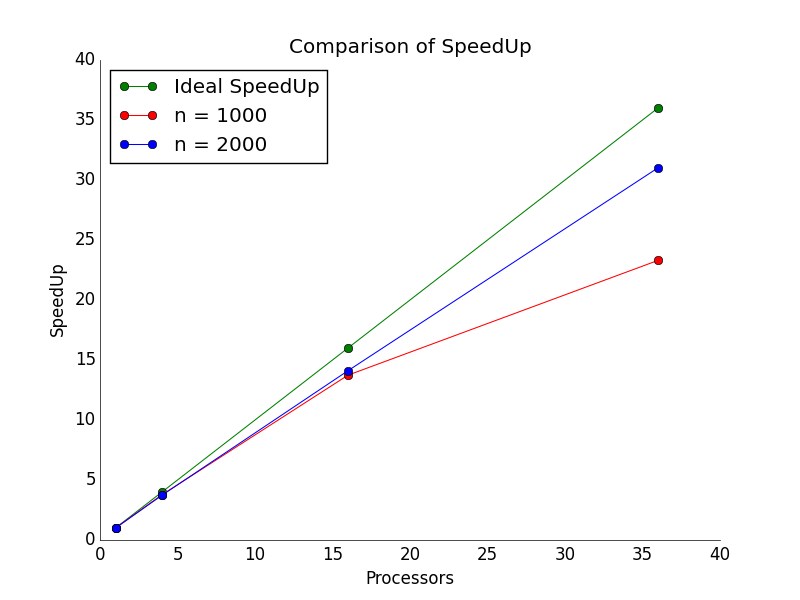
\includegraphics[width=.99\textwidth]{../2 Analysis/SpeedUp.png}
        \caption{Speed-Up}
        \label{fig:SpeedUp}
      \end{subfigure}%
      \begin{subfigure}{.5\textwidth}
        \centering
        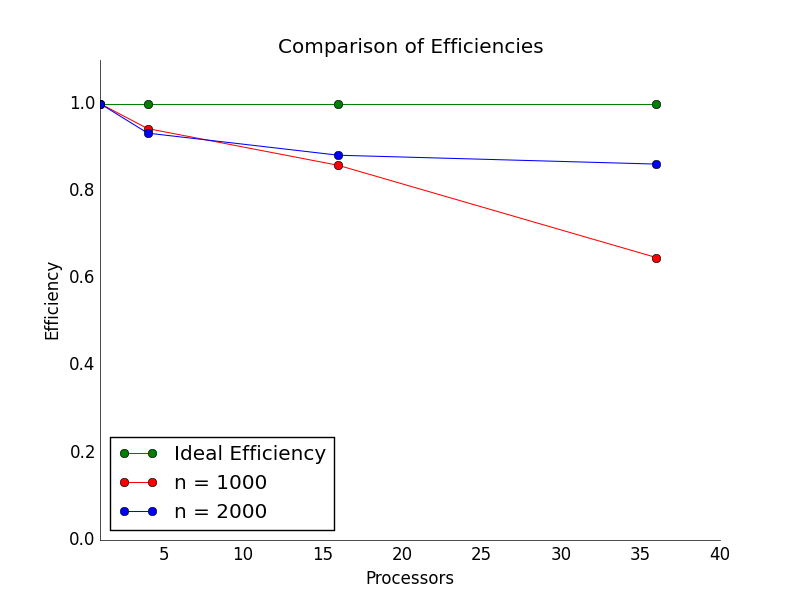
\includegraphics[width=.99\textwidth]{../2 Analysis/Efficiency.png}
        \caption{Efficiency}
        \label{fig:Efficiency}
      \end{subfigure}
      \caption{Speed-Up and Efficiency plots for the ideal case, $n=1000$ and $n = 2000$}
    \end{figure}


\newpage
\appendix
\section{Code}
    \lstinputlisting[caption = C++ code for the matrix algorithm, label = cod:matrix]{../Homework3/matrix.cpp}

\end{document}
